%%%%%%%%%%%%%%%%%%%%%%%%%%%%%%%%%%%%%%%%%%%
%THIS FILE CONTAINS ALL COMMON COMMANDS NEEDED FOR COMPILATION INTO BOTH PDF AND HTML.
%THE EXTENSION file src/macros.sty CONTAINS ONLY COMMANDS NEEDED EXCLUSIVELY FOR COMPILATION INTO PDF
%THE DIRECTORY src/hva/ CONTAINS ONLY COMMANDS NEEDED EXCLUSIVELY FOR COMPILATION INTO HTML WITH HEVEA, WITH THREE EXTENSION FILES, imakeidx.hva, macros.hva AND picins.hva.
%%%%%%%%%%%%%%%%%%%%%%%%%%%%%%%%%%%%%%%%%%%
% 2024/04:
% - \documentclass[] : change {book} to {scrbook} from KOMA-script -> rewritting the manual.
% - change fancyhdr to scrlayer-fancyhdr (compatibility with scrbook) to scrlayer-scrpage (contained in koma-script) -> modify macros.sty too.
% - rewriting title page for \maketitle (use with pandoc [produce html file], \begin(title)...\end(title) doesn't work with pandoc, "microtype" package too)
% 2024/10
% - renaming chapter files with an order number
% - clean documentclass / packages / add comments
% 2024/10
% - comment \ifIllustration to always have pictures in manuel
% - texlive-extra-utils -> make4ht
% 2024/11
% - simplification of \usepackage{graphicx} when pdf

%\ifx\pdfoutput\undefined		% if no pdfLaTeX outputting
% test KOMA-script with "scrbook" instead of "book"
%\documentclass[%
%	paper=a4,			% default=a4 and therefore not needed
%	12pt,				% default=11pt
%	headsepline,		% line under the header
%	footsepline,		% line above the footer
%	twoside=semi		% same left/right margins, default=twoside
%]{scrbook} 			% 
%}{
%\else							% else pdfLaTeX outputting
\documentclass[%
pdflatex,
a4paper,			% default=a4 and therefore not needed
12pt,				% default=11pt
english,			% use in babel, translator and varioref packages options %TODO: change with ngerman/english option in de/en manuals
toc=listof,			% add a "lof" (list of figures) line at the begining of the toc (table of contents)
twoside=semi,		% same recto/verso margins similar to simple verso margins, default=twoside
headsepline,		% draw rule below header
footsepline,		% draw rule above footer
plainfootsepline 	% draw footsepline on plain pages (here for heading pages, may be due to twoside=semi in scrbook options
]{scrbook} 				% KOMA-Script class "book"		
%}
%\fi

%\usepackage{ifpdf}					% detect pdfTeX, replaced by \Ifpdfoutput (KOMA-script)
\usepackage[T1]{fontenc}			% the font encoding
%\usepackage[utf8]{inputenc}			% no longer need to specify, included in LaTex since April 2018
\usepackage{lmodern}				% Latin Modern police
\usepackage{babel}					% use the language define in \documentclass
%\def\frenchcontentsname{Sommaire}	% rename "Table des matières" (at end of document) from [french]{babel} to "Sommaire" (at start of document)
%\frenchsetup{ItemLabeli=\textbullet}	% change 1st level list marker of french babel
%\frenchsetup{ItemLabelii=-}			% change 2nd level list marker of french babel
\usepackage{translator}		% for translating the Fixed Names
\usepackage{textcomp}				% for special characters like \textcurrency
%\usepackage{txfonts}
%\usepackage{ae}
%\usepackage{cmbright}
%\usepackage{times}					% changed from txfonts
\usepackage{newtxtext}				% install texlive-fonts-extra, replacing times which replaces txfonts
%\usepackage{lwarp}					% produce html file with lwarp (install texlive-extra-utils)

\usepackage{microtype}				% Font expansion (use for title) with "\textls[x]" - doesn't work with pandoc / espace entre caractères (utilisé pour le titre)
% Web addresses
%\usepackage{url}					% loaded by hyperref


% --------------------------------------------
% Load graphicx package with pdf if needed
% --------------------------------------------
%\ifpdf
%%\Ifpdfoutput{%
	%%\usepackage[pdftex]{graphicx}		% enhanced support for importing graphics (x=enhanced) and then using the \includegraphics command to insert the file
	%%}{%			
	% else								% Commented out to avoid errors in html, and put in the macros.sty file for pdf
	\usepackage{graphicx}				% enhanced support for importing graphics (x=enhanced) and then using the \includegraphics command to insert the file
	\newcommand{\refimage}[1]{ (fig. \vref{#1})}	% for the hypertext link display on images
	\newcommand{\vspacepdf}[1]{\vspace{#1}}			% for spaces after images bordered with text
	%%}
%% Graphics Extensions
%\ifpdf
%%\Ifpdfoutput{%
	%%\DeclareGraphicsExtensions{.pdf,.png,.jpg}
	%%}{%
	%\else
	%%\DeclareGraphicsExtensions{.eps}
	%%}
%\fi


% For illustrations
%\usepackage{picins}				% for text around image TODO change to wrapfig2 in the manuel
\usepackage{wrapfig2}				% TODO change in chapters, for text around image (replace picins)
\usepackage{caption}				% for good references in table of figures


%\usepackage{scrlayer-fancyhdr}		% facilities for constructing headers and footers, replace fancyhdr
% change to scrlayer-scrpage here and in macros.sty


%\pagestyle{fancyplain}
%\usepackage{tabularx}
%\usepackage{hhline}				% produce single or double line
%\usepackage{layout}				% TODO: Only if DE mode
\usepackage{varioref}		% defines the commands \vref, \vpageref, \vrefrange, and \vpagerefrange in french
%\usepackage{lastpage}
%\usepackage{longtable}
\usepackage{color}					% for a colored title page
%\usepackage{vmargin}				% for changing the title page margins
\usepackage{thumbpdf}				% create thumbnails (vignettes) in pdf


%\usepackage{emptypage}		% change by using \cleardoubleemptypage (in koma-scripts)
% Latex loads macros-3.0.sty for pdf output and Hevea loads /hva/macros.hva for html output
%\usepackage{macros-3.0}

%% Page layout %%
\usepackage[%
%	showframe,					% to see frame of geometry package
top=1in,					% marge haute
headheight=7mm,				% hauteur en-tête
headsep=6mm,				% distance entre entête et corps de texte
textheight=252mm,			% textheight=paperheight-topmargin-headheight-headsep-footskip
footskip=11mm,				% distance entre bas de pied de page et bas du corps de texte
hmargin=25mm				% horizontal margins (left and right), textwidth = paperwidt - margins
]{geometry}
\usepackage{scrlayer-scrpage}	% define and manage page styles by controlling page headers and footers			
\clearpairofpagestyles			% remove the default marks of the headings and the plain pages
\lehead{\leftmark}				% leftmark at left of even page
\lohead{\leftmark}				% leftmark at left of odd page
\rehead{\rightmark}				% rightmark at right of even page
\rohead{\rightmark}				% rightmark at right of odd page
\cfoot*{\pagemark}				% pagemark in the center of the footer
\ModifyLayer[addvoffset=-1ex]{scrheadings.foot.above.line}		% shift line up to increase distance between footer text and footerline in normal stylepages
\ModifyLayer[addvoffset=-1ex]{plain.scrheadings.foot.above.line}	% shift line up to increase distance between footer text and footerline in plain style page (chapter page)

%% Footnotes %%
\usepackage[%
perpage						% resets footnote numbering for each page of the document.
]{footmisc}						% provides several different customizations of footnotes

\renewcommand\footnoterule{%	% redefine rule above footnote
	\kern 5pt 					% above footnoterule, space between text and footnoterule  
	\hrule width 2.5in			% define rule's width to 2.5 in
	\kern 6pt					% space between footrule and footnotes below
}

%% Index %%
\usepackage[%
xindy						% sort index
]{imakeidx}						% for creating an index
\usepackage[%
columns=2,					% default value is 2
rule=1pt,					% thickness of a vertical rule between index columns. Default value is 0 pt, i. e. no rule.
totoc						% add index in toc
]{idxlayout}					% key-value interface to configure index layout parameters

\usepackage[unicode]{hyperref}		% replace \usepackage{url}, used to add an URL and rewrite the "grisbi-manuel-urldef.tex" file (must be the last package)
\hypersetup{%							% to create metadata to insert in pdf
	pdftitle={Manuel de Grisbi},		% sets the document information Title field
	pdfauthor={The Grisbi Team},		% sets the document information Author field
	pdfcreator={Alain PORTAL}			% sets the document information Creator field
	pdfpagemode=UseOutlines,			% set default mode of PDF display, UseOutlines=show bookmarks
	pdfstartview=XYZ null null 1.0,		% set the startup page view, XYZ=left top zoom
	pdffitwindow=true,					% resize document window to fit document size, default=false
	pdfcenterwindow=true,				% position the document window in the center of the screen, default=false
	bookmarksnumbered=true,				% put section numbers in bookmarks, default=false
	bookmarksopen=true,					% open up bookmark tree, default=false
	colorlinks=true,					% color links, default=false
	citebordercolor=1 1 1,				% the color of the box around citations, rgb color
	linkbordercolor=1 1 1,				% the color of the box around normal links, rgb color
	linkcolor=blue,						% color for normal internal links, color=blue
	menubordercolor=1 1 1,				% color of border around menu links, rgb color
	urlbordercolor=1 1 1,				% color of border around URL links, rgb color
	urlcolor=blue,						% color of URL links, color=blue
	plainpages=true					% do page number anchors as plain Arabic, default=false
%	pdfpagelabels=true					% set PDF page labels - Commenté car élimine  "Package hyperref Warning: Option `pdfpagelabels' has already been used,"
}
%%%%%%%%%%%%%%%%%%%%%%%%%%%%%%%%%%%%%%%%%%%%%%%%%%%%%%%%%%%%%%%
% Contents: The url chapter
% $Id: grisbi-manuel-urldef.tex, modified from previous file :
% $Id: grisbi-manuel-urldef.tex, v 0.8.8 2011/XX/XX Jean-Luc Duflot
% $Id: grisbi-manuel-urldef.tex, v 1.0 2014/02/12 Jean-Luc Duflot
% $Id: grisbi-manuel-urldef.tex, v 3.0 2024/04/07 Dominique Brochard: create
% $Id: grisbi-manuel-urldef.tex, v 3.0 2024/11 Dominique Brochard:
% - rename file to 31-xxx
% - modify \urldef{\urlListSF} to {\urlListDiffGrisbi}
% - update Martin Stromberger mail
%%%%%%%%%%%%%%%%%%%%%%%%%%%%%%%%%%%%%%%%%%%%%%%%%%%%%%%%%%%%%%%


\urldef{\urlGrisbi}%
\url{https://en.grisbi.org}

\urldef{\urlGrisbiTelechargement}%
\url{https://en.grisbi.org/post/Download}

\urldef{\urlBugTracker}%
\url{https://www.grisbi.org/bugsreports/}

\urldef{\urlGrisbiWiki}%
\url{https://github.com/grisbi/grisbi/wiki}

\urldef{\urlTuxFamily}%         % French website
\url{https://www.tuxfamily.org/en/main}

\urldef{\urlSourceForge}%
\url{https://sourceforge.net/projects/grisbi/files/}

\urldef{\urlSourceForgeDocumentation}%
\url{https://sourceforge.net/projects/grisbi/files/Documentation/}

\urldef{\urlGitHubGrisbi}%
\url{https://github.com/grisbi/grisbi/}

\urldef{\urlLinuxGraphic}%         % French website
\url{https://www.linuxgraphic.org}

\urldef{\urlFramasoftLogiciels}%         % French website
\url{https://framalibre.org/}

\urldef{\urlFreeSoftwareDirectory}%
\url{https://directory.fsf.org/wiki/Main_Page}

%\urldef{\urlAssociationsGouv}%
%\url{https://www.associations.gouv.fr/la-comptabilite-associative.html}

%\urldef{\urlPlanComptable}%
%\url{https://www.plancomptable.com/index.htm}

%\urldef{\urlPlanDeComptes}%
%\url{https://www.plancomptable.com/titre-IV/titre-IV_chapitre-III_section-1.htm#431-1}

%\urldef{\urlListeComptes}%
%\url{https://www.plancomptable.com/titre-IV/liste_des_comptes_sa.htm}

%\urldef{\urlMaisonAssociations}%
%\url{https://www.loi1901.com/regle_comptable.php}

%\urldef{\urlComptaOnLine}%
%\url{https://www.compta-online.com/plan-comptable-general-pdf-ao2428}

\urldef{\urlWikipedia}%
\url{https://en.wikipedia.org/}

\urldef{\urlMetonymyDef}%
\url{https://literarydevices.net/metonymy/}

%\urldef{\urlAndrePascualEmail}%
%\url{andre@linuxgraphic.org}% without the leading "mailto:" for the DVI version

%\urldef{\urlDanielCartronEmail}%
%\url{daniel@cartron.org}    % without the leading "mailto:" for the DVI version

%\urldef{\urlCedricAugerEmail}%
%\url{cedric@grisbi.org}     % without the leading "mailto:" for the DVI version

%\urldef{\urlSebastienBlondeelEmail}%
%\url{sbi@april.org}% without the leading "mailto:" for the DVI version

%\urldef{\urlGeraldNielEmail}%
%\url{gerald@grisbi.org}% without the leading "mailto:" for the DVI version

\urldef{\urlBenjaminDrieuEmail}%
\url{benjamin@drieu.org}     % without the leading "mailto:" for the DVI version

%\urldef{\urlDionysosEmail}%
%\url{dionysos@grisbi.org}     % without the leading "mailto:" for the DVI version

%\urldef{\urlJulietteEmail}%
%\url{juliette@grisbi.org}     % without the leading "mailto:" for the DVI version

\urldef{\urlFrancoisTerrotEmail}%
\url{grisbi@terrot.net}     % without the leading "mailto:" for the DVI version

%\urldef{\urlLoicBreillouxEmail}%
%\url{lbreilloux@users.sourceforge.net}    % without the leading "mailto:" for the DVI version

\urldef{\urlPierreBiavaEmail}%
\url{pierre.biava@orange.fr}     % without the leading "mailto:" for the DVI version

\urldef{\urlDidierChevalierEmail}%
\url{didier.chevalier35@gmail.com}     % without the leading "mailto:" for the DVI version

\urldef{\urlWilliamOllivierEmail}%
\url{guneeyoufix@gmail.com}     % without the leading "mailto:" for the DVI version

%\urldef{\urlMickaelRemarsEmail}%
%\url{grisbi@remars.com}     % without the leading "mailto:" for the DVI version

\urldef{\urlJeanLucDuflotEmail}%
\url{jielbil@mailo.com}     % without the leading "mailto:" for the DVI version

\urldef{\urlAlainLetientEmail}%
\url{al1.letient@free.fr}     % without the leading "mailto:" for the DVI version

%\urldef{\urlGuyLebegueEmail}%
%\url{guy@guy-lebegue.fr}     % without the leading "mailto:" for the DVI version

\urldef{\urlMicheleBondilEmail}%
\url{ciboulette05@club-internet.fr}     % without the leading "mailto:" for the DVI version

\urldef{\urlListInfoEmail}%
\url{info@listes.grisbi.org}     % without the leading "mailto:" for the DVI version

\urldef{\urlListDevelEmail}%
\url{devel@listes.grisbi.org}     % without the leading "mailto:" for the DVI version

\urldef{\urlLudovicRousseauEmail}%
\url{ludovic.rousseau@gmail.com}     % without the leading "mailto:" for the DVI version

\urldef{\urlDominiqueBrochardEmail}%
\url{dbro17@free.fr}     % without the leading "mailto:" for the DVI version

\urldef{\urlBobAndersonEmail}%
\url{www23@scilutions.co.uk}     % without the leading "mailto:" for the DVI version

\urldef{\urlMartinStrombergerEmail}%
\url{mstromberger@mailbox.org}     % without the leading "mailto:" for the DVI version

\urldef{\urlListTraductionEmail}%
\url{traduction@grisbi.org}  % without the leading "mailto:" for the DVI version

\urldef{\urlListBugsreport}%
\url{bugsreports@listes.grisbi.org}     % without the leading "mailto:" for the DVI version

\urldef{\urlListDiffGrisbi}%
\url{https://listes.grisbi.org/mailman/listinfo}     % without the leading "mailto:" for the DVI version


		% include the "grisbi-manuel-urldef" file during the compilation

%% Glossary %%
\usepackage[%
xindy,              % sort glossaries
toc                 % add the glossary reference to the toc (table of contents)
]{glossaries}       % create a glossary, must be loaded AFTER hyperref
\usepackage[%
automake
]{glossaries-extra} 	% check why no glossaries and give solutions

%% Index %%
\makeindex  %[intoc]	% creates the index with its reference in the toc

\definecolor{jaunegrisbi}{rgb}{1,1,.6}			% creating your own colors {yourcolorname}{model=rgb[0to1],RGB[0to255],cmyk or grey} rgb= 3 comma-separated values between 0 and 1 define the components of the color.
\definecolor{bleugrisbi}{rgb}{.1,.1,.4}
\definecolor{vertgrisbi}{rgb}{0,.6,.4}
\definecolor{ocregrisbi}{rgb}{1,.7,0}


% Virtualization of fonts
\newcommand{\lang}[1]{\emph{#1}}				% new command -> \lang = emph (e.g. italic)
\newcommand{\familyname}[1]{\textsc{#1}}		% new command -> \familynamelang = small caps
\newcommand{\menu}[1]{\textsl{#1}}				% new command -> \menu = slanted is oblique version of the roman font (e.g. italic)
\newcommand{\strong}[1]{\textsc{\textbf{#1}}}	% new command -> \strong = small caps + bold
\newcommand{\key}[1]{\texttt{<#1>}}				% new command -> \key = teletype font
\newcommand{\cmd}[1]{\texttt{#1}}				% new command -> \cmd = teletype font
\newcommand{\file}[1]{\textbf{#1}}				% new command -> \file = bold
\newcommand{\xml}[1]{\texttt{#1}}				% new command -> \xml = teletype font
\newcommand{\indexword}[1]{\textsf{#1}}			% new command -> \indexword = sans serif, for easy search of each indexed word in the page

%\renewcommand*{\footnote}{\centering}

\newcommand{\actuality}{}	% to see places to watch when updating the doc, using  the command grep actuality *.tex


%% Commented out because it doesn't work in html, and put in the macros.sty file for pdf
%% NE FONCTIONNE PAS POUR HTML
% redefine command listoffigures
%\ifpdf
%\makeatletter
%\renewcommand\listoffigures{%
%	% increases space between number and figure name for number >9 (see book.cls file)
%	\renewcommand\l@figure{\@dottedtocline{1}{1.5em}{2.8em}}%
%    \if@twocolumn
%     \@restonecoltrue\onecolumn
%    \else
%      \@restonecolfalse
%    \fi
%    \chapter*{\listfigurename}
%      \@mkboth{\MakeUppercase\listfigurename}{}
%    \@starttoc{lof}
%    \if@restonecol\twocolumn\fi
%    }
%\makeatother
%\else
%\fi

% For pdf only; for html, redefined  by an empty command in hva/macros.hva
% Glossary
\makeglossaries									% creates the glossary, entries of the glossary are in "src/{version}/{lang}/30-grisbi-manuel-glossary-en.tex"

%\input{grisbi-manuel-glossary}					% include "grisbi-manuel-glossary.tex" file in the document
\loadglsentries{30-grisbi-manuel-glossary-en}		% load and include glossary's entries in and from "30-grisbi-manuel-glossary-en"

%\input{grisbi-manuel-boolean-illustration}		% include "grisbi-manuel-boolean-illustration.tex" file in the document

%% -------------------
%% Begin of title page
%% -------------------

%\ifIllustration
\title{%
	\fontsize{40}{20}\selectfont					% increase size of title=40pt / line spacing=20pt
	\scshape										% small caps
	%	M\:a\:n\:u\:e\:l\; d\:e\; G\:r\:i\:s\:b\:i\\	% \: = medium space, \; = large space, \\ = line break
	\textls[250]{%									% increase space between characters, default=100 (active "microtype" package) [[ !!! doesn't work with pandoc !!! ]]
	Grisbi\; Manual}
	\\												% new line
	\vspace{1.5cm}									% vertical space between title and logo
	\includegraphics[width=6cm]{image/grisbi-logo.png}		% insert {file_name} graphic with width=6cm
	\vspace{1.5cm}									% % vertical space between logo and subtitle
}
\subtitle{%											% subtitle font size, default=large
	\sffamily\bfseries								% sans serif, bold
	\scshape										% small caps
	\fontsize{19}{20}\selectfont					% increase size of subtitle=20pt / line spacing=22pt
	Personal accounting software
	\vspace{1cm}\\									% vertical space
	\rule{4.5cm}{0.4pt}								% horizontal line, first argument width, second thickness
	\vspace{0.6cm}\\								% vertical space
}
\addtokomafont{author}{\large}						% modify author font size, default=Large
\author{%
	Copyright © 2001-2003 Daniel \familyname{Cartron}\\
	Copyright © 2004 Loïc \familyname{Breilloux}\\
	Copyright © 2004 Benjamin \familyname{Drieu}\\
	Copyright © 2011-2014 Jean-Luc \familyname{Duflot}\\
	Copyright © 2018 Bob \familyname{Anderson} (en)\\
	Copyright © 2018-2020 Martin \familyname{Stromberger} (de)\\
	Copyright © 2024 Dominique \familyname{Brochard}\\
	\rule{2.5cm}{0.4pt}							% insert horizontal line, first argument width, second thickness
}
\addtokomafont{date}{\large}					% modify date font size, default=Large
\date{%
	Version 3.0 of 2024 (provisional)
}
%\else
%\title{Manuel de Grisbi}
%\fi

%% -----------------
%% End of title page
%% -----------------

\begin{document}

%\pagestyle{scrheadings}			% titles of chapters and sections are repeated in the header, number of page in the footer


\maketitle							% create title page
%\cleardoubleoddemptypage			% force a break to an even (left, verso) page -> produce an additional odd page with empty style
% For pdf only; for html, redefined  by an empty command in hva/macros.hva
\frontmatter						% renders numbered pages in toc/tof in lower-case Roman letters

% not used
%\include{grisbi-manuel-title}

%\maketitle				% title v3.0.1 -> %\maketitle
%\myclearemptydoublepage

%\sommaire
\tableofcontents					% table of contents (toc)	

%\myclearemptydoublepage


% List of figures for pdf only ; for html, the addcontentsline is redefined by an empty command in hva/macros.hva
% Adds reference to lof in the toc
%\ifIllustration
%	\listoffigures
%		\ifpdf
%		\addcontentsline{toc}{chapter}{Table des figures}
%%		\myclearemptydoublepage
%		\cleardoubleemptypage % replace \myclearemptydoublepage
%		\else
%		\fi
%	\else
%\fi

\listoffigures				% list of figures (lof)

%% mis dans le \mainmatter pour lien correct des entrées d'index dans le préambule en html
%% voir aussi le chapitre Préambule
%\include{grisbi-manuel-preamble}
%\myclearemptydoublepage
% For pdf only; for html, redefined  by an empty command in hva/macros.hva
\mainmatter							% pages are numbered in Arabic numerals and the page counter is reset to 1.
%\KOMAScriptVersion						% print the used version number of Koma-Script
%\include{00-grisbi-manuel-preamble-en} 	 % TODO update screenshots and text "preamble", uncomment when finished
%\cleardoubleemptypage

%\include{01-grisbi-manuel-intro-en}			% TODO update screenshots and text "intro", uncomment when finished
%\cleardoubleemptypage

%\include{02-grisbi-manuel-entrance-en}		% TODO update screenshots and text "entrance", uncomment when finished
%\cleardoubleemptypage

%%%%%%%%%%%%%%%%%%%%%%%%%%%%%%%%%%%%%%%%%%%%%%%%%%%%%%%%%%%%%%%%%%
% Contents: The first start chapter
% $Id: grisbi-manuel-start.tex, v 0.4 2002/10/27 Daniel Cartron
% $Id: grisbi-manuel-start.tex, v 0.5.0 2004/06/01 Loic Breilloux
% $Id: grisbi-manuel-start.tex, v 0.6.0 2011/11/17 Jean-Luc Duflot
% $Id: grisbi-manuel-start.tex, v 0.8.9 2012/04/27 Jean-Luc Duflot
% $Id: grisbi-manuel-start.tex, v 1.0 2014/02/12 Jean-Luc Duflot
%%%%%%%%%%%%%%%%%%%%%%%%%%%%%%%%%%%%%%%%%%%%%%%%%%%%%%%%%%%%%%%%%


\chapter{Initial set-up of Grisbi\label{start}}


\section{Initial Set-up Wizard\label{start-first}}


After installing Grisbi, the first time the software is launched, it will help you with three consecutive wizards:

\begin{enumerate}
	\item The first wizard \enquote{Welcome to Grisbi!}, which will only appear once, on first launch, helps you configure the application. It comprises two steps, the second of which concerns management of the \indexword{account file}\index{account file} (automatic loading and saving, encryption and backup copies).

\begin{figure}[htbp]
	\begin{center}
		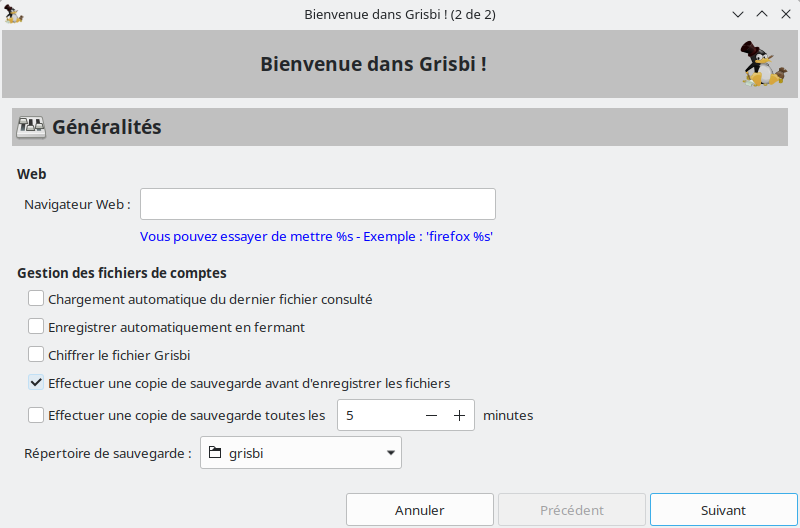
\includegraphics[width=0.98\textwidth]{image/screenshot/start_first_launch}
	\end{center}
	\caption{Initial configuration of accounts file.}
	\label{start_first_launch}
\end{figure}

It is advisable to check the options:
	\begin{itemize}
		\item Automatically load last file on startup%chargement automatique du dernier fichier consulté;
		\item Automatically save on exit;%enregistrer automatiquement en fermant;
		\item Make a backup copy before saving files (checked by default).%effectuer une copie de sauvegarde avant d'enregistrer les fichiers (coché par défaut).
	\end{itemize}
\end{enumerate}

\minisec{\textcolor{red}{\strong{Warning:}}}
The Grisbi developers recommend that you do not use the \menu{Encrypt Grisbi file} option for the following reasons:
\begin{itemize}
	\item there is no method for recovering an encrypted file whose password has been lost;
	\item For some unknown reason, using this option on Windows can render the accounts file completely unusable.
\end{itemize}  
However, if you use it, it is advisable to make regular back-ups of the unencrypted file.

\begin{enumerate}[resume]
	\item The second wizard, \enquote{Welcome to Grisbi!} (or later \enquote{New file Assistant}), which automatically follows the first, includes six steps to help you create the \indexword{account file}\index{account file}.%Le deuxième assistant \frquote{Bienvenue dans Grisbi !} (ou plus tard \frquote{Aide à la création d'un nouveau fichier de comptes}), qui suit automatiquement le premier, comprend six étapes qui vous aiderons à la création du \indexword{fichier de comptes}\index{fichier de comptes}.
	\item This is followed automatically by the third wizard, \enquote{Create a new account}, which is used to create the first account and is described in detail in section \ref{start-newfile} below.%Puis vient automatiquement le troisième assistant \frquote{Créer un nouveau compte} qui permet de créer le premier compte et qui est décrit en détail dans la section \ref{start-newfile} ci-dessous.
\end{enumerate}

At any time you can exit any wizard with the \menu{Cancel} button.

If you do not want to use the Set-up Wizard, you can open a example file instead (see the next section \ref{start-example} below).



\section{Example file\label{start-example}}


If you want to use Grisbi immediately without having to go through the full set-up, for example to get an idea of the possibilities of this program, you can download the  \file{Example\_3.0-en.gsb} file from \lang{Sourceforge.net}\footnote{\urlSourceForgeDocumentation{}} website in the folder \enquote{textsf{examples}}.

% espace avant Attention ou Note :  mm
\vspacepdf{5mm}
\textbf{Note}: in this example file, the names of the payees etc are pure invention; any similarity with a real person or business is entirely accidental.

\section{Creation of a new set of accounts\label{start-newfile}}


The first time you use Grisbi, you will need to create a first
\indexword{accounts file}\index{accounts file}. The \gls{extension} of this file will be \file{.gsb} and its name will be \file{your-file-name.gsb}.

% TODO update below

Immediately afterwards, you will need to create at least one account, and then some other accounts (current accounts, savings, credit, possibly a cash account and some transition accounts) that will contain their respective transactions.

For personal accounting, you will normally have only one account file, as this supports all the links between your different accounts. If you manage a busniess, or another personal account without a financial relationship with the first one, you will create another account file, which will have another name \file{your-second-file.gsb}. Thus \indexword{accounting entities}\index{accounting entity} will remain well separated.


% espace avant Attention ou Note : 5 mm
\vspacepdf{5mm}

\strong{Caution}: for a given reporting entity, it is necessary and important to distinguish between the  \enquote{\indexword{accounts file}\index{accounts file}} and the  \enquote{\indexword{account files}\index{account files}}:
\begin{itemize}

\item The \enquote{accounts file} you have created will have the extension \file{.gsb} and the name of \file{your-file.gsb}; it contains all the data of all the accounts created for the management of an accounting entity;

\item The \enquote{account files} are files that you may need to use or create to import or export data from one accounting application to another; these files will only contain data from one account (current or otherwise) at a time; they will have different extensions (\file{.ofx}, \file{.csv} or \file{.qif}) depending on their content; for more details, see the chapter \vref{move}, \menu{Export and import of accounts}.
\end{itemize}

% espace aprs Attention ou Note: 5 mm
\vspacepdf{5mm}
In other words, all the accounts in your household accounts are recorded in a single accounts file, and all the accounts in your business are stored in a separate accounts file; and an account in Grisbi can correspond to an account file, but only when talking about importing or exporting data.

% espace pour changement de thme
\vspacepdf{5mm}

The general procedure for creating an account file is as follows: click on the menu File - New Account File; the account file creation wizard opens, which includes six steps. In the sixth step, the assistant offers you:

\begin{itemize}
\item  create a new account, and then follow the account creation wizard, which itself includes five steps, to create the first account (because it is essential to have at least one account);
\item or to use pre existing data, then use the import wizard, which also includes five steps, to import existing account operations.
\end{itemize}

After creating this first account or importing existing account transactions, if you want to create other accounts, you will return to the end of the process of creating the account file, which will return you in both cases to the create a new account option.


% espace pour changement de thme
\vspacepdf{5mm}
To create your accounts file, click the File - New Account File menu; the detailed procedure is as follows:
enumerate
welcome window: confirm with the Forward button;

To create your accounts file, click the \menu{File - New Account File} menu: the detailed procedure is as follows:

\begin{enumerate}
\item New file assistant welcome window: confirm with the \menu{Forward} button:
\item General configuration
générale\refimage{start-file-create-img}:




\begin{figure}[htbp]
\begin{center}
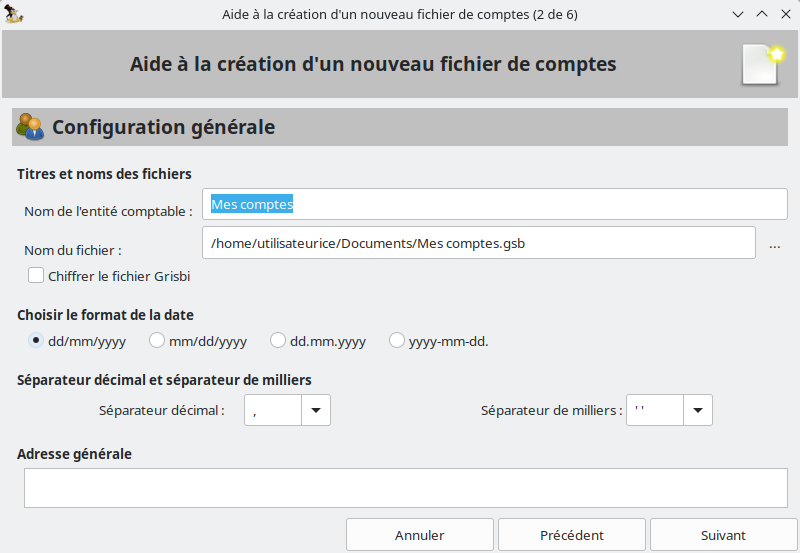
\includegraphics[scale=0.5]{image/screenshot/start_file_create}
\end{center}
\caption{General configuration of an account file}
\label{start-file-create-img}
\end{figure}



\begin{enumerate} 
 \item choose the name of the accounting entity whose accounts you are managing, for example \enquote{My accounts}, which can be chosen as the title of the Grisbi application home page,
\item enter the name of the accounts file with its complete tree; Grisbi defaults to the same name as the reporting entity, but you can change it
\item check the  \menu{Encrypt Grisbi} box if you wish \gls{to encrypt} the accounts file,
\item select the \indexword{date format}\index{date format} with one of the two buttons: dd/mm/yyyy for day/month/year, or  mm/dd/yyyy for month/day/year,
\item choose the decimal \indexword{separator}\index{separator} and the thousands from the drop-down lists,
 \item fill in the address (optional),
 \item  confirm with the  \menu{Forward} button;
\end{enumerate}

\item selection of the base \indexword{currency}\index{currency}:
\begin{enumerate} 
 \item click on the chosen currency in the list,
\item check the "include obsolete currencies" box if you also want to display old currencies,
\item confirm with the \menu{Forward} button;
\end{enumerate}

\item selection of the  \indexword{list of categories}\index{catgories !types} you will use:
\begin{enumerate} 
 \item click on your desired category, either the \menu{Standard category list} or the \menu{Empty list} \footnote{\strong{Translators Note:} Users installing the program on a system with a French Language interface will find different categories are offered including some for business users} 
\item check the \menu{Display foreign category sets} box to check if other categories are available\footnote{\strong{Translators Note:} This option is mainly for the benefit of users of a computer system with the French Language interface who will then be shown the two English categories mentioned in the previous step}
\item confirm with the \menu{Forward} button;
\end{enumerate}

\item Enter details of \indexword{banks}\index{banques !définition} holding your accounts:
\begin{enumerate} 
 \item click  \menu{Add} to define a bank; fill in the details of the bank (name, bank code, etc.), then confirm with the \menu{Add} to add the bank,
\item select a bank from the list and click the \menu{Remove} button to delete a bank, then confirm in the window that opens,
\item repeat actions a and b as many times as necessary,
\item  confirm with the \menu{Forward}  button to go to the next step, \menu{Creating a new account}:
\end{enumerate} 

\item configuration completed: the configuration of the accounts file is complete, and this window offers you to choose one of the two methods of creating your first account
compte\refimage{start-account-choice-img}:


\begin{figure}[ht]
\begin{center}
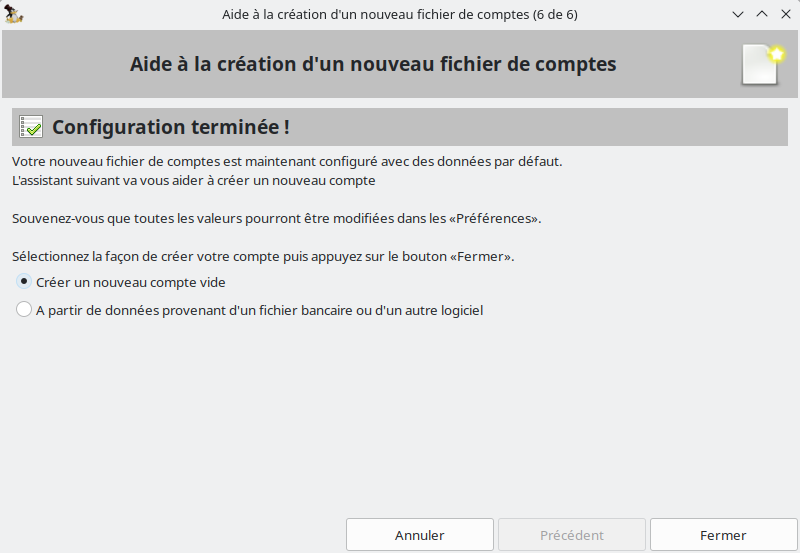
\includegraphics[scale=0.5]{image/screenshot/start_account_choice}
\end{center}
\caption{Selecting the first account}
\label{start-account-choice-img}
\end{figure}


\begin{itemize}
\item \menu{Create a new empty account}: if you check this line, then if you confirm with the \menu{Close} button, this window closes and the new account creation wizard starts. See  \vref{accounts-new}, \menu{Creating a new account},  which fully describes this procedure, then return to this page:

\item \menu{From data from a bank file or other software}: if you check this line and then confirm with the \menu{Close} button ,  this window closes and the Import Data Wizard of a file account by Grisbi starts. See the \vref{move-import-importinit} section, \menu{Importing Account Files from Another Programme into Grisbi}, which fully describes this procedure, then return to this page.
\end{itemize}
\end{enumerate}

% tiquette du paragraphe suivant, pour que les liens hypertexte dans account.tex et QIF.tex  arrivent bien dessus
\label{start-newfile-end}

\textit{\textbf{In one way or another}}, you have now created your accounts file, as well as the first account of this file.

%espace pour changement de thme
\vspacepdf{5mm}

If you want to create other accounts now, select the \menu{Edit - New Account} to create another account (see the \vref{accounts-new}, \menu{ Creating a new account} section).

%espace pour changement de thme
\vspacepdf{5mm}

Otherwise, you can start using the account you just created or the one from which you just imported the data.

% espace avant Attention ou Note : 5 mm
\vspacepdf{5mm}

\strong{Warning}: in general, it is inadvisable to have accents or spaces in the names of directories and files used by Grisbi. If so, rename them now. For example, spaces can be replaced by underscores (\underline{}).

% saut de page pour titre solidaire
\newpage


\section{Saving your accounts file\label{start-save}}

Your operations are not written as you enter them as they might be in other software; you must therefore save your account file before exiting. Do not worry, Grisbi warns you if you have not done so.

You can configure the options for saving the account file in the  \menu{ Edit - Preferences} menu, see the section \vref{setup-general-files-manage}, \menu{Managing Account Files.}.


\section{Import from other personal accounting software}

See the \vref{move-import-importinit} section to import account files from another program into Grisbi. For the moment, Grisbi supports \gls{Gnucash}, \gls{OFX}, \GLS{CSV} and \GLS{QIF} formats.


			% TODO update screenshots and text "start", uncomment when finished
%\cleardoubleemptypage

%\include{05-grisbi-manuel-home-en}			% TODO update screenshots and text "home", uncomment when finished
%\cleardoubleemptypage

%\include{06-grisbi-manuel-QIF-en}			% TODO update screenshots and text "QIF", uncomment when finished
%\cleardoubleemptypage

%\include{07-grisbi-manuel-datamanagement-en}	% TODO update screenshots and text "datamanagement", uncomment when finished
%\cleardoubleemptypage

%\include{08-grisbi-manuel-accounts-en}		% TODO update screenshots and text "accounts", uncomment when finished
%\cleardoubleemptypage

%\include{09-grisbi-manuel-transactions-en}	% TODO update screenshots and text "transactions", uncomment when finished
%\cleardoubleemptypage

%\include{10-grisbi-manuel-reconciliation-en}	% TODO update screenshots and text "reconciliation", uncomment when finished
%\cleardoubleemptypage

%\include{11-grisbi-manuel-planned-en}		% TODO update screenshots and text "planned", uncomment when finished
%\cleardoubleemptypage

%\include{12-grisbi-manuel-search-en}			% TODO update screenshots and text "search", uncomment when finished
%\cleardoubleemptypage

%\include{13-grisbi-manuel-third-en}			% TODO update screenshots and text "third", uncomment when finished
%\cleardoubleemptypage

%\include{14-grisbi-manuel-categories-en}		% TODO update screenshots and text "categories", uncomment when finished
%\cleardoubleemptypage

%\include{15-grisbi-manuel-budgetlines-en}	% TODO update screenshots and text "budgetlines", uncomment when finished
%\cleardoubleemptypage

%\include{16-grisbi-manuel-financialyear-en}	% TODO update screenshots and text "financialyear", uncomment when finished
%\cleardoubleemptypage

%\include{17-grisbi-manuel-credit-en}			% TODO update screenshots and text "credit", uncomment when finished
%\cleardoubleemptypage

%\include{18-grisbi-manuel-budget-en}			% TODO update screenshots and text "budget", uncomment when finished
%\cleardoubleemptypage

%\include{19-grisbi-manuel-bankcardmanagement-en}	% TODO update screenshots and text "bankcardmanagement", uncomment when finished
%\cleardoubleemptypage

%\include{20-grisbi-manuel-association}		% fr version only
%\cleardoubleemptypage

%\include{21-grisbi-manuel-reports-en}			% TODO update screenshots and text "reports", uncomment when finished
%\cleardoubleemptypage

%\include{22-grisbi-manuel-reports-creation-en}	% TODO update screenshots and text "reports-creation", uncomment when finished
%\cleardoubleemptypage

%\include{23-grisbi-manuel-setup-en}				% TODO update screenshots and text "setup", uncomment when finished
%\cleardoubleemptypage

%\include{24-grisbi-manuel-maintenance-en}		% TODO update screenshots and text "maintenance", uncomment when finished
%\cleardoubleemptypage



%% Files editors not used anymore, so useless 
%%\include{grisbi-manuel-todo}
%%\cleardoubleemptypage
%
%% Files editors not used anymore, so useless 
%%\include{grisbi-manuel-problems}
%%\cleardoubleemptypage
%
%% Useless so don't include it
%%\include{grisbi-manuel-XML}
%
%% Useless so don't include it
%%\include{grisbi-manuel-FDL}


% Prints the index
\printindex


% Displays a note at the beginning of the glossary
\renewcommand{\glossarypreamble}{\textbf{Note}: most of the definitions in this glossary are taken from articles of the same name in the free, collaborative encyclopaedia \lang{Wikipédia}
\footnote{\urlWikipedia{}}. Although these texts have been modified and adapted to the specific context of this glossary, the author would like to thank Wikipedia for providing these references.\newline}


% Prints the glossary
% For pdf only; redefined in hva/macros.hva by an empty command in html
\printglossaries


\end{document}



